\scanpage{20}
\mspage{8}
It amounts to the same to say that $\sigma_0,\sigma_1,\sigma_\infty,\rho$ are generators, with defining relations
\[
(4)\qquad
(\overbrace{\rho^{-1}\sigma_\infty\sigma_0\deleted{\rho}}^{l_\infty})
(\overbrace{\rho^{-1}\sigma_1\sigma_\infty\deleted{\rho}}^{l_1})
(\overbrace{\rho^{-1}\sigma_0\sigma_1\deleted{\rho}}^{l_0})=1
\]
\[
(5)\qquad \sigma_0^2=\sigma_1^2=\sigma_\infty^2=1
\]
\[
(6)\qquad \rho^3=1
\]
\margin{One must add the relations $\rho\sigma_0\rho^{-1}=\sigma_1$ etc
One has two generators $\sigma_0,\rho$ in fact with relations
\[
\sigma_0^2=\rho^3=1,
\]
the
\deleted{$\unsure{[\underset{\sigma_\infty}{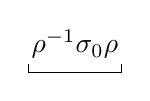
\begin{tikzpicture}[baseline=(term.base)]\node[inner sep=1pt] (term) {$\rho^{-1}\sigma_0\rho$};\draw ([yshift=-1pt]term.south west) -- ++(0,-3pt) -| ([yshift=-1pt]term.south east);\end{tikzpicture}}\sigma_0\rho^{-1}][\underset{\sigma_1}{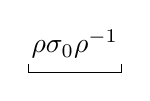
\begin{tikzpicture}[baseline=(term.base)]\node[inner sep=1pt] (term) {$\rho\sigma_0\rho^{-1}$};\draw ([yshift=-1pt]term.south west) -- ++(0,-3pt) -| ([yshift=-1pt]term.south east);\end{tikzpicture}}\underset{\sigma_\infty}{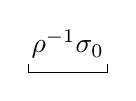
\begin{tikzpicture}[baseline=(term.base)]\node[inner sep=1pt] (term) {$\rho^{-1}\sigma_0$};\draw ([yshift=-1pt]term.south west) -- ++(0,-3pt) -| ([yshift=-1pt]term.south east);\end{tikzpicture}}\rho^{-1}]|[\underset{\sigma_\infty}{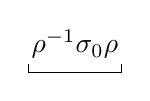
\begin{tikzpicture}[baseline=(term.base)]\node[inner sep=1pt] (term) {$\rho^{-1}\sigma_0\rho$};\draw ([yshift=-1pt]term.south west) -- ++(0,-3pt) -| ([yshift=-1pt]term.south east);\end{tikzpicture}}\sigma_0\rho^{-1}][\underset{\sigma_1}{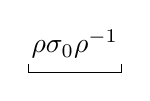
\begin{tikzpicture}[baseline=(term.base)]\node[inner sep=1pt] (term) {$\rho\sigma_0\rho^{-1}$};\draw ([yshift=-1pt]term.south west) -- ++(0,-3pt) -| ([yshift=-1pt]term.south east);\end{tikzpicture}}\underset{\sigma_\infty}{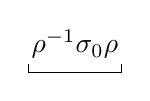
\begin{tikzpicture}[baseline=(term.base)]\node[inner sep=1pt] (term) {$\rho^{-1}\sigma_0\rho$};\draw ([yshift=-1pt]term.south west) -- ++(0,-3pt) -| ([yshift=-1pt]term.south east);\end{tikzpicture}}\rho^{-1}]}$}
relation (4) is a consequence of the preceding ones (comes from the fact $\sigma_1=\rho\sigma_0\rho^{-1}$, \deleted{\illegible{1}} $\sigma_\infty=\rho^{-1}\sigma_0\rho$). Note that
\[
\begin{aligned}
l_0&=\deleted{\unsure{(\rho\sigma_0\rho^{-1})^2|(\sigma_0\rho)^2}}\rho^{-1}(\sigma_0\rho)^2\rho
=\boxed{\rho^{-1}\sigma_0\rho\sigma_0\rho^{-1}}\\
l_1&=(\deleted{\unsure{\rho}}\sigma_0\rho)^2\\
l_\infty&=(\unsure{\rho^{\deleted{-1}}|\rho^{-1}}\sigma_0\deleted{\unsure{\rho}})^2
\end{aligned}
\]
\[
\begin{aligned}
\operatorname{int}(\sigma_0)l_1&=l_\infty\\
\operatorname{int}(\sigma_0)l_\infty&=l_1\\
\operatorname{int}(\sigma_0)(l_0)&=l_\infty^{-1}l_1^{-1}
\end{aligned}
\]}
\margin{\uline{NB}
\[
\begin{aligned}
\sigma_0(l_0)&=l_\infty^{-1}l_1^{-1}\\
\sigma_0(l_1)&=l_\infty\\
\sigma_0(l_\infty)&=l_1^{\deleted{\unsure{-1}}}\deleted{\unsure{l_\infty^{-1}|l_0^{-1}}}
\end{aligned}
\]
and ditto for $\sigma_1,\sigma_\infty$}
\uline{NB} If one sets \inserted{in addition} $\sigma_0,\sigma_1,\sigma_\infty=1$ in it, one finds as defining relation $\rho^3=1$, \deleted{\unsure{thus}} nothing more, which proves that $\rho$ is not a word \unsure{p.v.|with respect to} the $\sigma_i$\ldots

All this is compatible with the relations from the beginning, \deleted{\unsure{if in the latter one had taken everything with primes}, and \unsure{one interprets} $l_i'=l_i^{-1}$, $\sigma_i'=\sigma_{\unsure{\dot\rho(i)}}$}
\deleted{i.e. $\sigma_i$} \deleted{\unsure{of our group|so that} $\unsure{\mathcal E'|\sigma_i'|\sigma'}$} if one replaces the $l_i$ by the $l_i^{-1}$ there
Here one has, since $\sigma_i=\sigma^{\unsure{\prime|1}}_{\dot\rho^{-1}(i)}$
\[
(7)\quad\left\{\begin{aligned}
\operatorname{int}(\sigma_i)&:\text{ exchanges }l_j\text{ and }l_{\deleted{\unsure{j}}k}
\quad\inserted{(i,j,\unsure{k|h})\text{ distinct})}\ \deleted{\text{and}}\\[-2pt]
&\deleted{\text{(and the }\unsure{\text{last}|\text{becoming}}\ l_{\dot\rho(i)}\ \text{is deduced from it by (1))}}\\
\operatorname{int}(\rho)l_i&=l_{\dot\rho(i)}
\end{aligned}\right.
\]

One would now like to make explicit the $\varepsilon_i$ with $\varepsilon_i^2=l_i$ $(i=0,1,\infty)$, $\varepsilon_i$ being \unsure{thus a|one of the} \unsure{generators|generator} \unsure{of the|of the} centralizer (or normalizer, it is the same) of the $L_i$ in $\mathcal E^+$\unsure{.|,} (or the centralizer in $\mathcal E$). The calculations made above, with the changes of \unsure{notation|notations} indicated, give
\[
\deleted{(8)}\quad\left\{\begin{aligned}
\unsure{\deleted{\varepsilon_0}|\varepsilon_0}&=l_0^{\deleted{\unsure{-1|4}}}\sigma_1 l_{\unsure{0|1}}^{\deleted{\unsure{-1|4}}}\\
\unsure{\deleted{\varepsilon_1}|\varepsilon_1}&=\unsure{\deleted{l_\infty^{-1}}|l_\infty^{-1}}\sigma_\infty \deleted{l_1^{-1}}\ \inserted{l_1}\\
\varepsilon_\infty&=l_0^{-1}\sigma_0 l_\infty
\end{aligned}\right.
\]
\mspage{19}
